\documentclass[11pt, a4paper,titlepage]{article}
	\usepackage[spanish]{babel}
	\selectlanguage{spanish}
	\usepackage[utf8]{inputenc} % Aca va el setup para el codigo.
    \usepackage{graphicx}
	\usepackage{alltt} %Esto no lo necesitamos
    \usepackage{upquote}% esto tampoco creo
    \usepackage{listings}
	\usepackage{mdframed}
	\usepackage{xcolor} 
    \usepackage[utopia]{mathdesign}
\newmdtheoremenv[% ACA PODES MODIFICAR LAS PROPIEDADES DEL CODIGO {code}
font=\fontsize{12pt}{16pt},
linecolor=gray,leftmargin=-2.6cm,%
rightmargin=-2.6cm,
backgroundcolor=gray!5,%
innertopmargin=8pt,%
ntheorem]{code}{Codigo}[section]
%-----------------------------------------------------------
\begin{document}  %Aqui empieza el documento
\begin{titlepage} %Esta es la caratula
\centering
{\scshape\Huge Un curso de gráficos para iniciados del Matlab\par}
\vspace{1cm}
\begin{figure}[h]
\centering
\includegraphics[width=7cm]{logo/asme.png}
\end{figure}
\vspace{2cm}
{\scshape\Large\textbf{Autores} \par}
\medskip %medskip,smallskip,vspace son todos comandos para dejar espacio en blanco entre cosas
 \textsc{\large Canalis - 56674 \\ Whittingslow - 11-3953-0963\\ \textit{{\tiny Call me!}} }

\end{titlepage} %Termina la caratula
\section{Subploteando}
%\includegraphics[width=\textwidth]{1zunch.pdf}

\begin{code}
\begin{verbatim}

A=[1:10].^2;
B=randi(11,20,1);
C=randi([8,10],10,3);
tufuncion=@(x)cos(3*x)*x;

subplot(2,3,1),plot(A,':g')
grid on
subplot(2,3,2),plot(B,'y*')
subplot(2,3,3),fplot(tufuncion,[0,2*pi],'--k')
subplot(2,3,4),plot(C)
title('2-D Line Plot')
xlabel('x')
ylabel('cos(5x)')
ylim([7,11])
\end{verbatim}% las mierditas de los apostrofes joden mucho.
\end{code}
\begin{figure}[h]
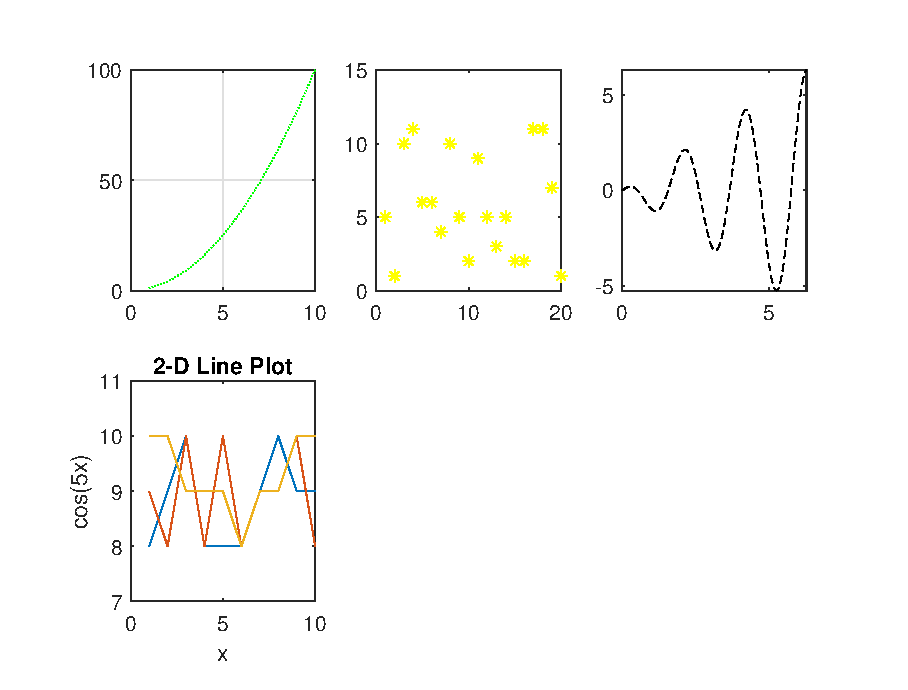
\includegraphics[width=\textwidth]{graf/g3.eps}

\end{figure}
\section{Manipulación de imágenes} 
\subsection{Colormap}
\begin{code}
\begin{verbatim}

colormap('default');
Matriz1=randi(64,50,100); %Hay 64 colores en el colormap
image(Matriz1)
\end{verbatim}
\end{code}

\begin{figure}[h]
\centering
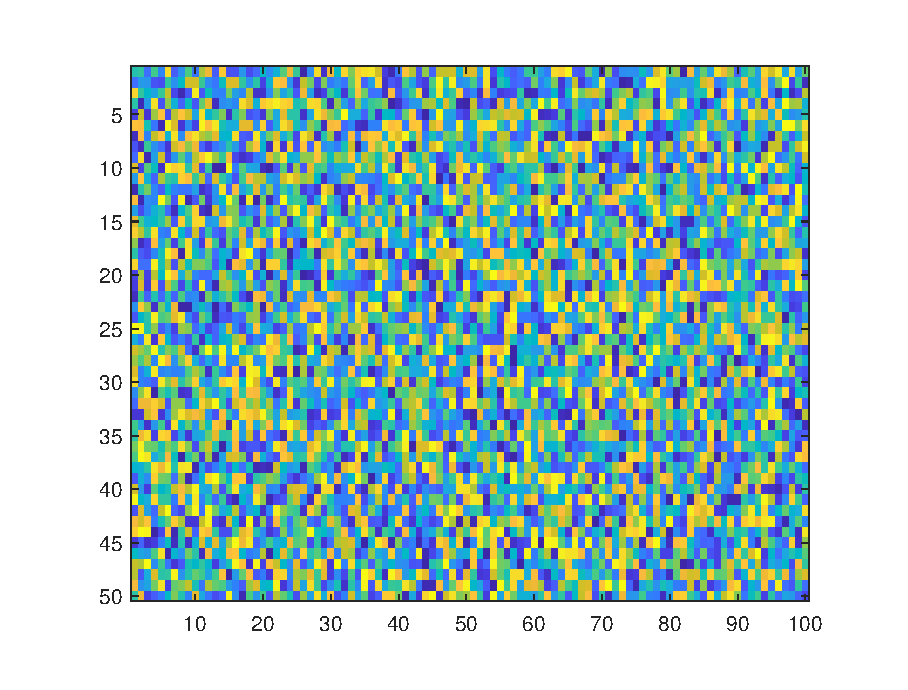
\includegraphics[width=10cm]{graf/g4_1.eps}
\end{figure}

\begin{code}
\begin{verbatim}

figure %Inicializa el grafico
colormap([0,0,0;0.5,0.5,0.5;1,1,1]) 
  %Las filas son los distintos colores
  %(valores en RGB) En este caso, negro, gris, blanco
Matriz2=randi([1,3],34); 
  %Esta matriz de 34x34 tiene indices 
  %que refieren a las filas del colormap
image(Matriz2)
\end{verbatim}
\end{code}
\clearpage
\begin{figure}[h]
\centering
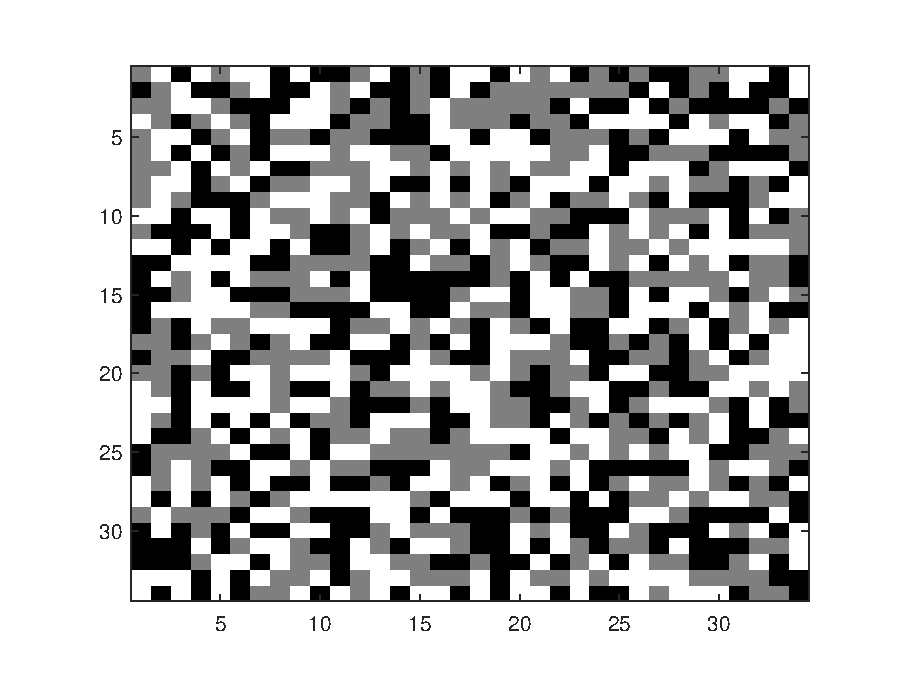
\includegraphics[width=10cm]{graf/g4_2.eps}
\end{figure}
\subsection{Windows.jpg}
\begin{code}
\begin{verbatim}

figure
Matriz3=imread('windows.jpg'); %Esta matriz de
  %1200x1920x3 con numeros del 0 al 255 
  %Tiene los valores RGB para cada pixel
Matriz3(200:400,:,2)=255; %puedo modificar la matriz como
  %siempre. Hago que color verde sea máximo en esta zona
Matriz3(:,1200:1400,:)=[];%Corto una franja vertical
  %de 1400-1200 pixeles
image(Matriz3)

\end{verbatim}
\end{code}
\clearpage

\begin{figure}[h]
\centering
\includegraphics[width=\textwidth]{graf/g4_3.eps}
\end{figure}
\subsection{Guardar imagen a archivo}
\begin{code}
\begin{verbatim}

SoyElMapa=winter;
imwrite(Matriz1,SoyElMapa,'TuNombreParaImagen.png') 
   %Guarda la imagen en formato
   %png, que si bien es pesado, no pierde información
   %Los otros formatos también están disponibles
\end{verbatim}
\end{code}
\clearpage
\section{Simbolos y Labels}
\begin{code}
\begin{verbatim}

load n5_datos.mat
fig=figure;   
    %Genero el diagrama y lo guardo como fig para editar despues
blk=[0 0 0];  %Guardo el color negro en blk
set(fig,'defaultAxesColorOrder',[blk; blk])
    %cambio color de ejes
semilogx(rev,fev1,'b-')
hold on            
semilogx(rev,fev2,'r-')
semilogx(rev,fev3,'c-') 
semilogx(rev,fev4,'y-')
yl=ylim;    %Guarda los limites del eje para tener referencia
    %cuando haya un nuevo eje y
title('Mi Gran Grafico')
xlabel('Valor Independiente \delta')
ylabel('Valor Dependiente \epsilon')
yyaxis right      
%Crea un nuevo eje y queda como eje activo
yticks('manual')  
%Esto va permitir modificar los ticks del nuevo eje
yticks([fev1(end),fev2(end),fev3(end),fev4(end)]) 
%Guarda posiciones de los ticks
ylim(yl)                
%Iguala limites del nuevo eje al del primer eje
yticklabels({'Azul!' , 'Rojo!', 'Celeste!' ,'Amarillo!'})
ylabel('Los Colores del Arco iris \heartsuit')
grid on
\end{verbatim}
\end{code}
\clearpage
\begin{figure}[h]
\centering
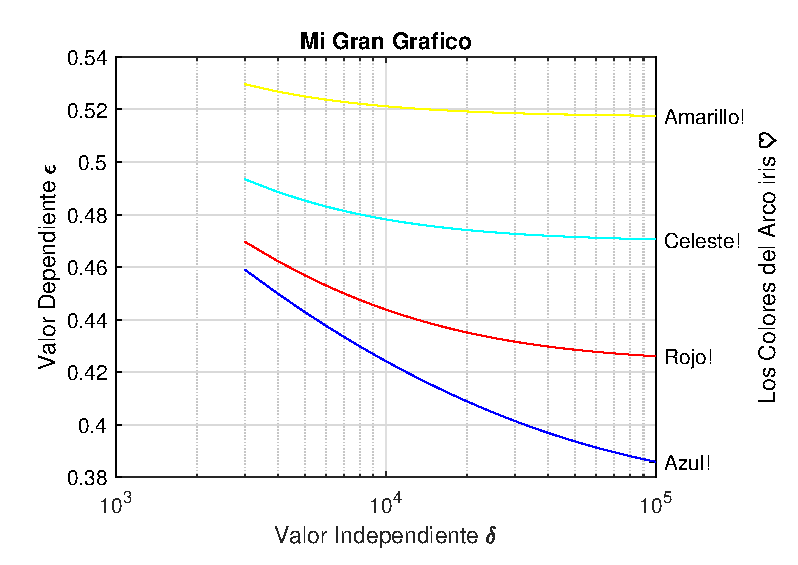
\includegraphics[width=\textwidth]{graf/g5_rev.eps}
\end{figure}
\section{\LaTeX\space y {\scshape Matlab}}
\begin{code}
\begin{verbatim}

syms x y %Para trabajar con la funcion latex 
    %de matlab hay que declarar los
    %variables que se van a usar como simbolicos
valoresZ=peaks(100); 
    %Devuelve 100x100 valores de la
    %funcion prueba de Matlab
xval=1:100;
yval=1:100;
surf(xval,yval,valoresZ); 
    %Grafico la superficie de peaks con un mapa 100x100
z =  3*(1-x)^2*exp(-(x^2) - (y+1)^2) ... 
   - 10*(x/5 - x^3 - y^5)*exp(-x^2-y^2) ... 
   - 1/3*exp(-(x+1)^2 - y^2); 
   %Funcion graficada (es peaks)
title(['La ecuacion:$'latex(z)'$'],'Interpreter','latex')
    %Pongo lo que se va hacer pasar por el compilador
    %de LaTex entre los corchetes
xlabel('Con \LaTeX Todo es Mejor','Interpreter','latex')
\end{verbatim}
\end{code}
\begin{figure}[h]
\centering
\includegraphics[width=\textwidth]{graf/g6.eps}
\end{figure}
% \begin{code}

% La linea de abajo es para 
% \begin{verbatim}

% %   Tome los terminos de sumatoria en string o funcion anonima. Usar t y n.
% \end{verbatim}
% \end{code}
\end{document} 

